\chapter{Overview\label{chap:1_hand_tracking_overview}}

In this Part we present a solution to the difficult problem of inferring the continuous pose of a human hand. We do so by first constructing an accurate database of labeled ground-truth data in an automatic process, and then training a system capable of real-time inference using ConvNets. Since the human hand represents a particularly difficult kind of articulable object to track, we believe our solution is applicable to a wide range of articulable objects. Our method has a small latency equal to one frame of video, is robust to self-occlusion, requires no special markers, and can handle objects with self-similar parts (i.e. fingers). To allow a broad range of applications, our method works when the hand is smaller than 2\% of the $640\times480$px image area.

Traditionally, commercial motion capture solutions have not included infrastructure to infer hand pose and instead focus on full-body skeletal animation. This is largely due to the difficulty that arises because articulable objects - like the human hand - have many DOF, constrained parameter spaces, self-similar parts, and suffer from self-occlusion. For this work we utilize a depth camera since it provides a dense set of accurate measurements of the physical geometry of the hand, however even with this high dimensional input modality, inferring the pose is still difficult because of data loss due to ``dropped-pixels'' (an artifact of the depth sensing device) and self occlusion.

One common approach to ``fill in'' missing data is to combine multiple simultaneous video streams; but this is a costly demand on the end-user and may prohibit widespread use of otherwise good solutions. A second common approach, called ``supervised learning'' in computer vision and machine learning, is to train a model on ground-truth data, which combines the full pose of the object in the frame with the depth image. The trained model can then use a priori information from known poses to make informed guesses about the likely pose in the current frame.

Large ground-truth datasets have been constructed for important articulable objects such as human bodies. Unfortunately, most articulable objects, even common ones such as human hands, do not have publicly available datasets, or these datasets do not adequately cover the vast range of possible poses. Perhaps more importantly, it may be desirable to infer the real-time continuous pose of objects that do not yet have such datasets. The vast majority of objects seen in the world fall into this category, and a general method for dataset acquisition of articulable objects is an important contribution of this work.

The main difficulty with using supervised learning for training models to perform real-time pose inference of a human hand is in obtaining ground-truth data for hand pose. Typical models of the human hand have 25-50 degrees of freedom ~\cite{erol2007vision} and exclude important information such as joint angle constraints. Since real hands exhibit joint angle constraints that are pose dependent, faithfully expressing such limits is still difficult in practice. Unfortunately, without such constraints, most models are capable of poses which are anatomically incorrect. This means that sampling the space of possible parameters using a real hand is more desirable than exploring it with a model. With the advent of commodity depth sensors, it is possible to economically capture continuous traversals of this constrained low-dimensional parameter space in video, and then robustly fit hand models to the data to recover the pose parameters~\cite{bmvc2011oikonom}.

\begin{figure}[ht]
\centering
\includegraphics[width=0.8\columnwidth]{figures_1_hand_tracking/overview.pdf}
    \caption{Pose Recovery Pipeline Overview}
    \label{fig:overview}
\end{figure}

Our method can be generalized to track any articulable object that satisfies three requirements: 1) the object to be tracked can be modeled as a 3D boned mesh, 2) a binary classifier can be made to label the pixels in the image belonging to the object, and 3) the projection from pose space (of the bones) to a projected 2D image in depth is approximately one-to-one. 

An overview of this pipeline is shown in Figure~\ref{fig:overview} and the output of each stage is shown in Figure~\ref{fig:overview_detail}. The 3D boned mesh of the articulable object is used to automatically label depth video captured live from a user. This data is used to train a Randomized Decision Forest (RDF) architecture for image segmentation (output shown in Figure~\ref{fig:overview_detail_a}), create a comprehensive database of depth images with ground-truth pose labels (output shown in Figure~\ref{fig:overview_detail_b}), which is then used to train a ConvNet to infer the position of key model features in real-time (output shown in Figure~\ref{fig:overview_detail_c}). We also suggest a simple and robust inverse kinematics (IK) algorithm for real-time, high degree of freedom pose inference from the ConvNet output (output shown in Figure~\ref{fig:overview_detail_d}). 

Note that our system can accommodate multiple commodity depth cameras for generating training data, but requires only a single depth camera for real-time tracking.

\begin{figure}[ht]
\centering
        % trim option's parameter order: left bottom right top
	\subcaptionbox{\footnotesize RDF classification\label{fig:overview_detail_a}}{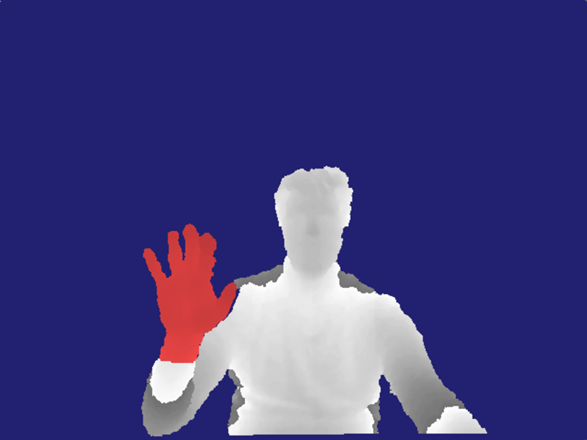
\includegraphics[height=3.7cm, trim = 20mm 0mm 30mm 22.5mm, clip]{figures_1_hand_tracking/overview_1}}
	\subcaptionbox{\footnotesize Model Fitting\label{fig:overview_detail_b}}{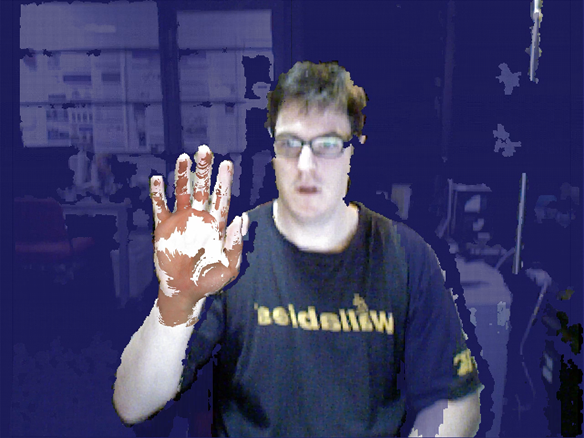
\includegraphics[height=3.7cm, trim = 15mm 0mm 20mm 5mm, clip]{figures_1_hand_tracking/overview_2}}
        \subcaptionbox{\footnotesize ConvNet Inference\label{fig:overview_detail_c}}{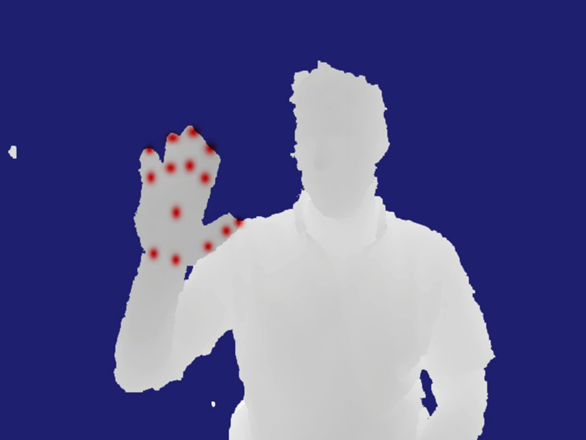
\includegraphics[height=3.7cm, trim = 15mm 0mm 20mm 5mm, clip]{figures_1_hand_tracking/overview_3}}
        \subcaptionbox{\footnotesize IK\label{fig:overview_detail_d}}{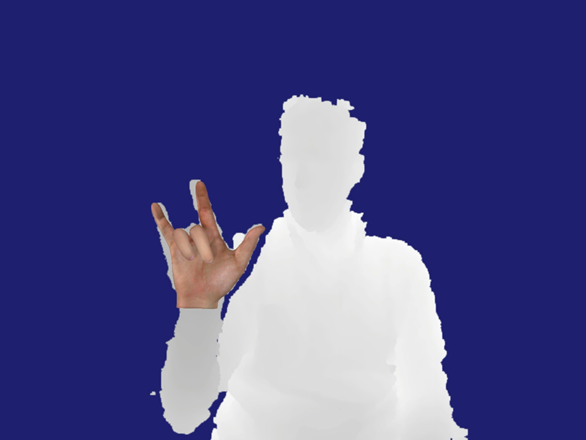
\includegraphics[height=3.7cm, trim = 20mm 0mm 15mm 10mm, clip]{figures_1_hand_tracking/overview_4}}
        \caption{Pipeline Stage Outputs}
        \label{fig:overview_detail}
\end{figure}

As a single example, training our system on an open-source linear-blend-skinning model of a hand with 42 degrees of freedom takes less than 10 minutes of human effort (18,000 frames at 30fps), followed by two days of autonomous computation time. Tracking and pose inference for a person's hand can then be performed in real-time using a single depth camera. Throughout our experiments, the camera is situated in front of the user at approximately eye-level height. The trained system can be readily used to puppeteer related objects such as alien hands, or real robot linkages, and as an input to 3D user interfaces~\cite{Stein2012}.

\chapter{Hand Tracking Architecture\label{chap:1_hand_tracking_archiecture}}

\section{Binary Classification}
\label{sec:binary_classification}

For the task of hand-background depth image segmentation we trained an RDF classifier to perform per-pixel binary segmentation on a single image. The output of this stage is shown in Figure \ref{fig:rdf_data}. Decision forests are well-suited for discrete classification of body parts~\cite{shotton2013real}. Furthermore, since decision forest classification is trivially parallelizable, it is well-suited to real-time processing in multi-core environments.

\begin{figure}[ht]
\centering
        \begin{subfigure}{0.4\textwidth}
                \centering
                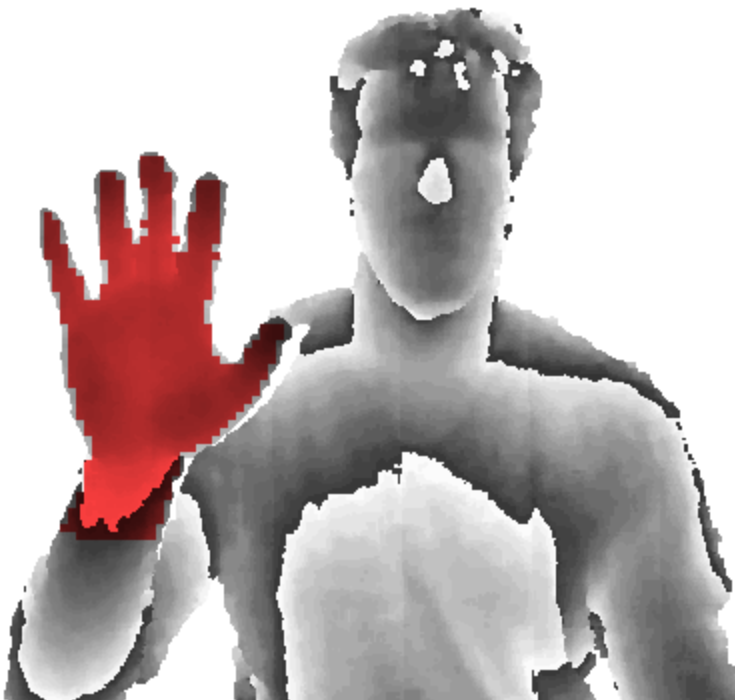
\includegraphics[width=\textwidth]{figures_1_hand_tracking/decision_forest_downsampled_labels_cropped}
                \caption{\footnotesize Ground-Truth Labels}
        \end{subfigure}
        \begin{subfigure}{0.4\textwidth}
                \centering
                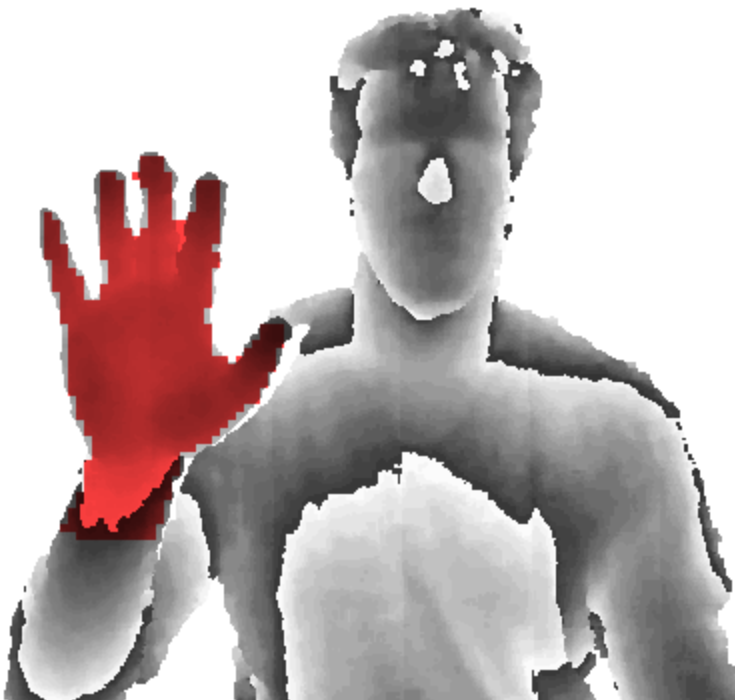
\includegraphics[width=\textwidth]{figures_1_hand_tracking/decision_forest_generated_labels_cropped}
                \caption{\footnotesize Labels Inferred by RDF}
        \end{subfigure}
        \caption{Decision Forest Data: learned labels closely match target}
        \label{fig:rdf_data}
\end{figure}

After Shotton et al., our RDF is designed to classify each pixel in a depth image as belonging to a hand or background. Each tree in the RDF consists of a set of sequential deterministic decisions, called weak-learners (or nodes), that compare the relative depth of the current pixel to a nearby pixel located at a learned offset. The particular sequence of decisions a pixel satisfies induces a tentative classification into hand or background. An overview of the RDF architecture is shown in Figure~\ref{fig:rdf_overview}. For each pixel in the image, the algorithm starts at the root of each Randomized Decision Tree (RDT) and proceeds down the left or right sub-trees according to the binary decision made by the weak-learner at each node.  The leaf nodes describe the distribution of labels in the training set for the pixels that satisfy the weak-learner sequence. Averaging the classification from all trees in the forest induces a final probability distribution for each pixel, where the inferred label is taken as the argmax of the distribution. As our implementation differs only slightly from that of Shotton et al., we refer interested readers to their past work, and focus on the innovations particular to our implementation.

\begin{figure}[ht]
\centering
\includegraphics[width=0.8\columnwidth]{figures_1_hand_tracking/RDF}
    \caption{RDF Overview}
    \label{fig:rdf_overview}
\end{figure}

While full body motion capture datasets are readily available~\cite{Allen2003}, these datasets either lack articulation data for hands or else do not adequately cover the wide variety of poses that were planned for this system. Therefore, it was necessary to create a custom database of full body depth images with binary hand labeling for RDF training (Figure \ref{fig:rdf_data}). We had one user paint their hands bright red with body paint and used a simple HSV-based distance metric to estimate a coarse hand labeling on the RGB image. The coarse labeling is then filtered using a median filter to remove outliers. Since commodity RGB+Depth (RGBD) cameras, typically exhibit imperfect alignment between depth and RGB, we used a combination of graph cut and depth-sensitive flood fill to further clean up the depth image labeling~\cite{Boykov}.

In order to train the RDF we randomly sample weak-learners from a family of functions similar to \cite{shotton2013real}. At a given pixel $(u,v)$ on the depth image $I$ each node in the decision tree evaluates:
\begin{equation}
    I\left(u + \frac{\Delta u}{I\left(u,v\right)}, v + \frac{\Delta v}{I\left(u,v\right)}\right) - I\left(u,v\right)\geq d_{t}
    \label{eq:rdf}
\end{equation}
Where $I\left(u,v\right)$ is the depth pixel value in image $I$, $\Delta u$ and $\Delta v$ are learned pixel offsets, and $d_{t}$ is a learned depth threshold. Experimentally, we found that (\ref{eq:rdf}) requires a large dynamic range of pixel offsets during training to achieve good classification performance. We suspect that this is because a given decision path needs to use both global and local geometry information to perform efficient hand-background segmentation. Since training time is limited, we define a discrete set of weak-learners that use offset and threshold values that are linear in log space and then we randomly sample weak-learners from this space during training.

\section{Dataset Creation}
\label{sec:datasetcreation}

The goal of this stage is to create a database of RGBD sensor images representing a broad range of hand gestures with accurate ground-truth estimates (i.e. labels) of joint parameters in each image that may be used to train a ConvNet. The desired ground-truth label consists of a 42-dimensional vector describing the full degree of freedom pose for the hand in that frame. The DOF of each hand-joint is shown in Figure \ref{fig:libhand}. After the hand has been segmented from the background using the RDF-based binary classification just described, we use a direct search method to deduce the pose parameters based on the approach of Oikonomidis et al.~\cite{bmvc2011oikonom}. An important insight of our work is that we can capture the power of their direct search method in an offline fashion, and then use it to train ConvNets (or similar  algorithms) that are better suited to fast computation. One advantage of this decoupling is that during offline training we are not penalized for using more complicated models, which are more expensive to render, and which better explain the incoming range data. A second advantage is that we can utilize multiple sensors for training, thereby mitigating problems of self-occlusion during real-time interaction with a single sensor.

\begin{figure}[ht]
\centering
\includegraphics[width=0.4\textwidth]{figures_1_hand_tracking/libhand.pdf}
    \caption{Linear Blend Skinning (LBS) Model~\protect\cite{libhand} with 42 DOF}
    \label{fig:libhand}
\end{figure}

The algorithm proposed by Oikonomidis et al.~\cite{bmvc2011oikonom} and adopted with modifications for this work is as follows; starting with an approximate hand pose, a synthetic depth image is rendered and compared to the depth image using an scalar objective function. This depth image is rendered in an OpenGL-based framework, where the only render output is the distance from the camera origin and we use a camera with the same properties (e.g. focal length) as the PrimeSense IR sensor. In practice the hand pose is estimated using the previous frame's pose when fitting a sequence of recorded frames. The pose is manually estimated using a simple UI for the first frame in a sequence. This results in a single scalar value representing the quality of the fit given the estimated pose coefficients. The particle swarm optimization with partial randomization (PrPSO) direct search method~\cite{PRPSO} is used to adjust the pose coefficient values to find the best fit pose that minimizes this objective function value. An overview of this algorithm is shown in Figure \ref{fig:pso_architecture}.

\begin{figure}[ht]
\centering
\includegraphics[width=0.6\textwidth]{figures_1_hand_tracking/dataset_generation.pdf}
    \caption{Algorithm Pipeline For Dataset Creation}
    \label{fig:pso_architecture}
\end{figure}

Since PSO convergence is slow once the swarm positions are close to the final solution (which is exacerbated when partial randomization is used to prevent premature swarm collapse on early local minima), we then use a robust variant of the Nelder-Mead optimization algorithm~\cite{Tseng95fortified-descentsimplicial} after PSO has completed. The Nelder-Mead optimization algorithm is a simplex-based direct-search optimization algorithm for non-linear functions. We have found that for our optimization problem, it provides fast convergence when sufficiently close to local optima.

Since this dataset creation stage is performed offline, we do not require it to be fast enough for interactive frame rates. Therefore we used a high-quality, linear-blend-skinning (LBS) model~\cite{libhand} (shown in Figure \ref{fig:libhand}) as an alternative to the simple ball-and-cylinder model of Oikonomidis et al. After reducing the LBS model's face count to increase render throughput, the model contains 1,722 vertices and 3,381 triangle faces, whereas the high density source model contained 67,606 faces. While LBS fails to accurately model effects such as muscle deformation and skin folding, it represents many geometric details that ball-and-stick models cannot.

To mitigate the effects of self-occlusion we used three sensors (at viewpoints separated by approximately 45 degrees surrounding the user from the front), with attached vibration motors to reduce IR-pattern interference~\cite{shake_n_sense} and whose relative positions and orientations were calibrated using a variant of the Iterative Closest Point (ICP) algorithm~\cite{Horn87closed-formsolution}. While we use all three camera views to fit the LBS model using the algorithm described above, we only use depth images taken from the center camera to train the ConvNet. The contributions from each camera were accumulated into an overall fitness function $F\left(C\right)$, which includes two \emph{a priori} terms ($\Phi\left(C\right)$ and $P\left(C\right)$) to maintain anatomically correct joint angles as well as a data-dependent term $\Delta(I_s, C)$ from each camera's contribution. The fitness function is as follows:

\begin{equation}
    F\left(C\right)=\sum_{s=1}^3\bigg(\Delta(I_s, C)\bigg) + \Phi\left(C\right) + P\left(C\right)
    \label{eq:pso_func}
\end{equation}

Where $I_s$ is the $s$ sensor's depth image and $C$ is a 42-dimensional coefficient vector that represents the 6 DOF position and orientation of the hand as well as 36 internal joint angles (shown in Figure \ref{fig:libhand}). $P\left(C\right)$ is an interpenetration term (for a given pose) used to invalidate anatomically incorrect hand poses and is calculated by accumulating the interpenetration distances of a series of bounding spheres attached to the bones of the 3D model. We define interpenetration distance as simply the sum of overlap between all pairs of interpenetrating bounding spheres. $\Phi\left(C\right)$ enforces a soft constraint that coefficient values stay within a predetermined range ($C_{\text{min}}$ and $C_{\text{max}}$):

\begin{equation*}
    \Phi\left(C\right) = \sum\limits_{k=1}^n w_k\left[\operatorname{max}\left(C_k-C_{k\text{max}}, 0\right) + \operatorname{max}\left(C_{k\text{min}}-C_k, 0\right)\right]
    \label{eq:pso_penalty}
\end{equation*}

Where, $w_k$ is a per-coefficient weighting term to normalize penalty contributions across different units (since we are including error terms for angle and distance in the same objective function). $C_{\text{min}}$ and $C_{\text{max}}$ were determined experimentally by fitting an unconstrained model to a discrete set of poses which represent the full range of motion for each joint. Lastly $\Delta(I_s, C)$ of Equation (\ref{eq:pso_func}), measures the similarity between the depth image $I_s$ and the synthetic pose rendered from the same viewpoint:

\[
    \Delta\left(I_s,C\right)=\sum_{u,v}\operatorname{min}\left(\left|I_s(u,v)-R_s(C,u,v)\right|,d_{\text{max}}\right)
    \label{eq:pso_depth_compare}
\]

Where, $I_s(u,v)$ is the depth at pixel $(u,v)$ of sensor $s$, $R_s(C,u,v)$ is the synthetic depth given the pose coefficient C and $d_{\text{max}}$ is a maximum depth constant. The result of this function is a clamped L1-norm pixel-wise comparison. It should be noted that we do not include energy terms that measure the silhouette similarity as proposed by Oikonomidis et al. since we found that when multiple range sensors are used these terms are not necessary.

Since the same pose is seen by multiple cameras from different viewpoints, it is necessary to calculate an affine transformation from each camera's viewpoint into a consistent basis. Due to variations in the imaging systems of each camera, small three-dimensional scale variations are common across views of the same object. For this reason, classical iterative closest point (ICP) with scale ~\cite{Horn87closed-formsolution} is insufficient for our needs, and instead we use a straightforward weighted variant of ICP based on energy minimization. In this variant, for an arbitrary 3D point in the data $p_j$, and the corresponding closest point $q_j$ on the model, we minimize the overall discrepancy of the fit $E$, given the current camera to world coordinate transformation $T_i$ (for each camera $i$), as follows:

\begin{align}
E = \sum_{i=1}^N\sum_{j=1}^Mw_j\left\|T_iq_j - p_j\right\|^2 \nonumber \\
w_j = \frac{\operatorname{max}\left(0, \frac{\text{dot}(\hat{q_j}, \hat{p_j}) - k}{ 1 - k}\right)}{1 + \left\|p_j-q_j\right\|} \nonumber
\end{align}

Where there are $N+1$ cameras and $M$ points in our system. The per-correspondence weight $w_j$ biases the fit towards points that are already close and have normals $\hat{p_j},\hat{q_j}$ pointing in the same direction. The resulting fit is mostly insensitive to the constant $k \in (0,1)$, and we used $k = 0.5$. Using suitable calibration geometry and a known approximate initial transformation, the above algorithm converges within 50 to 100 iterations using BFGS to perturb the parameters of the affine matrices $T_i$.

\section{Feature Detection}
\label{sec:realtimefeaturedetection}

We employ a multi-resolution, deep ConvNet architecture inspired by the work of Farabet et al.~\cite{Farabet} in order to perform feature extraction of 14 salient hand points from a segmented hand image. Since depth images of hands tend to have many repeated local image features (for instance fingertips), ConvNets are well suited to perform feature extraction since multi-layered feature banks can share common features, thereby reducing the number of required free parameters.

We recast the full hand-pose recognition problem as an intermediate collection of easier individual hand-feature recognition problems, which can be more easily learned by ConvNets. In early experiments we found inferring mappings between depth image space and pose space directly (for instance measuring depth image geometry to extract a joint angle), yielded inferior results to learning with intermediate features. We hypothesize that one reason for this could be that learning intermediate features allows ConvNets to concentrate the capacity of the network on learning local features, and on differentiating between them. Using this framework the ConvNet is also better able to implicitly handle occlusions; by learning compound, high-level image features the ConvNet is able to infer the approximate position of an occluded and otherwise unseen feature (for instance, when making a fist, hidden finger-tip locations can be inferred by the knuckle locations).

We trained the ConvNet architecture to generate an output set of \emph{heat-map} feature images (Figure \ref{fig:heat_maps}). Each feature heat-map can be viewed as a 2D Gaussian (truncated to have finite support), where the pixel intensity represents the probability of that feature occurring in that spatial location. The Gaussian UV mean is centered at one of 14 feature points of the user's hand. These features represent key joint locations in the 3D model (e.g., knuckles) and were chosen such that the inverse kinematics (IK) algorithm described in Section \ref{sec:realtimeposedetection} can recover a full 3D pose.

\begin{figure}[ht]
\centering
\includegraphics[width=\textwidth]{figures_1_hand_tracking/heat_maps_2_feat.pdf}
    \caption{Depth image overlaid with 14 feature locations and the heat-map for two fingertip features.}
    \label{fig:heat_maps}
\end{figure}

We found that the intermediate heat-map representation not only reduces required learning capacity but also improves generalization performance since failure modes are often recoverable. Cases contributing to high test set error (where the input pose is vastly different from anything in the training set) are usually heat-maps that contain multiple hotspots. For instance, the heat-map for a fingertip feature might incorrectly contain multiple lobes corresponding to the other finger locations as the network failed to discriminate among fingers. When this situation occurs it is possible to recover a reasonable feature location by simple heuristics to decide which of these lobes corresponds to the desired feature (for instance if another heat-map shows higher probability in those same lobe regions then we can eliminate these as spurious outliers). Similarly, the intensity of the heat-map lobe gives a direct indication of the system's confidence for that feature, which is an extremely useful measure for practical applications.

Our multi-resolution ConvNet architecture is shown in Figure \ref{fig:cnn}. The segmented depth image is initially pre-processed, whereby the image is cropped and scaled by a factor proportional to the mean depth value of the hand pixels, so that the hand is in the center and has size that is depth invariant. The depth values of each pixel are then normalized between 0 and 1 (with background pixels set to 1). The cropped and normalized image is shown in Figure \ref{fig:heat_maps}.

\begin{figure}[ht]
\centering
\includegraphics[width=0.9\textwidth]{figures_1_hand_tracking/CNN_architecture.pdf}
    \caption{Convolutional Network Architecture}
    \label{fig:cnn}
\end{figure}

The preprocessed image is then filtered using local contrast normalization~\cite{JarrettLeCun}, which acts as a high-pass filter to emphasize geometric discontinuities. The image is then down-sampled twice (each time by a factor of 2) and the same filter is applied to each image. This produces a multi-resolution band-pass image pyramid with 3 banks (shown in Figure \ref{fig:pyramid}), whose total spectral density approximates the spectral density of the input depth image. Since experimentally we have found that hand-pose extraction requires knowledge of both local and global features, a single resolution ConvNet would need to examine a large image window and thus would require a large learning capacity; as such a multi-resolution architecture is very useful for this application.

\begin{figure}[ht]
\centering
        \begin{subfigure}{0.3\textwidth}
                \centering
                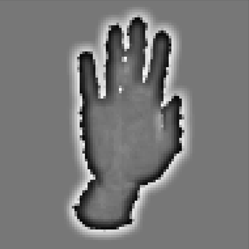
\includegraphics[width=\textwidth]{figures_1_hand_tracking/pyramid1}
                \caption{\footnotesize 96$\times$96px}
        \end{subfigure}
        \begin{subfigure}{0.3\textwidth}
                \centering
                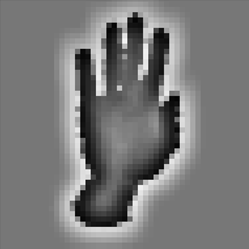
\includegraphics[width=\textwidth]{figures_1_hand_tracking/pyramid2}
                \caption{\footnotesize 48$\times$48px}
        \end{subfigure}
        \begin{subfigure}{0.3\textwidth}
                \centering
                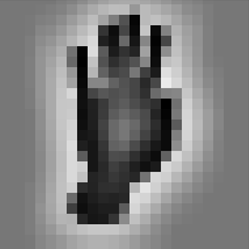
\includegraphics[width=\textwidth]{figures_1_hand_tracking/pyramid3}
                \caption{\footnotesize 24$\times$24px}
        \end{subfigure}
        \caption{Neural Network Input: Multi-Resolution Image Pyramid}
        \label{fig:pyramid}
\end{figure}

The pyramid images are propagated through a 2-stage ConvNet architecture. The highest resolution feature bank is shown in Figure \ref{fig:feature_detector}. Each bank is comprised of 2 convolution modules, 2 piecewise non-linearity modules, and 2 max-pooling modules. Each convolution module uses a stack of learned convolution kernels with an additional learned output bias to create a set of output feature maps (please refer to \cite{LeCunMNIST} for an in-depth discussion). The convolution window sizes range from 4x4 to 6x6 pixels. Each max-pooling~\cite{nagi} module sub-samples it's input image by taking the maximum in a set of non-overlapping rectangular windows. We use max-pooling since it effectively reduces computational complexity at the cost of spatial precision. The max-pooling windows range from 2x2 to 4x4 pixels. The nonlinearity is a Rectify Linear Unit (ReLU), which has been shown to improve training speed and discrimination performance in comparison to the standard sigmoid units~\cite{ImageNet_NIPS2012_0534}. Each ReLU activation module computes the following per-pixel non-linear function:

\begin{equation*}
    f\left(x\right)=\operatorname{max}\left(0,x\right)
\end{equation*}

\begin{figure}[ht]
\centering
\includegraphics[width=0.85\textwidth]{figures_1_hand_tracking/feature_detector.pdf}
    \caption{High-Resolution Bank Feature Detector: (each stage: Nfeats,height,width)}
    \label{fig:feature_detector}
\end{figure}

Lastly, the output of the ConvNet banks are fed into a 2-stage neural network shown in Figure \ref{fig:linear_network}. This network uses the high-level convolution features to create the final 14 heat-map images; it does so by learning a mapping from localized convolution feature activations to probability maps for each of the bone features. In practice these two large and fully-connected linear networks account for more than 80\% of the total computational cost of the ConvNet. However, reducing the size of the network has a very strong impact on runtime performance. For this reason, it is important to find a good tradeoff between quality and speed. Another drawback of this method is that the neural network must implicitly learn a likelihood model for joint positions in order to infer anatomically correct output joints. Since we do not explicitly model joint connectivity in the network structure, the network requires a large amount of training data to perform this inference correctly.

\begin{figure}[ht]
\centering
\includegraphics[width=0.65\textwidth]{figures_1_hand_tracking/linear_network.pdf}
    \caption{2-Stage Neural Network To Create The 14 Heat Maps (with sizing of each stage shown)}
    \label{fig:linear_network}
\end{figure}

ConvNet training was performed using the open-source machine learning package Torch7~\cite{torch7}, which provides access to an efficient GPU implementation of the back-propagation algorithm for training neural networks. During supervised training we use stochastic gradient descent with a standard L2-norm error function, batch size of $64$ and the following learnable parameter update rule:

\begin{align}
    %\gamma_i = \operatorname{max}\left(\gamma_{min},\gamma_0-k\left(i-1\right)\right) \nonumber \\
    \Delta w_i = \gamma\Delta w_{i-1}-\lambda\left(\eta w_i-\frac{\partial L}{\partial w_i}\right) \nonumber \\
    w_{i+1} = w_i + \Delta w_i
\end{align}

Where $w_i$ is a bias or weight parameter for each of the network modules for epoch $i$ (with each epoch representing one pass over the entire training-set) and $\frac{\partial L}{\partial w_i}$ is the partial derivative of the error function $L$ with respect to the learnable parameter $w_i$ averaged over the current batch. We use a constant learning rate of $\lambda = 0.2$, and a momentum term $\gamma=0.9$ to improve learning rate when close to the local minimum. Lastly, an L2 regularization factor of $\eta=0.0005$ is used to help improve generalization.

During ConvNet training the pre-processed database images were randomly rotated, scaled and translated to improve generalization performance~\cite{Farabet}. Not only does this technique effectively increase the size of the training set (which improves test / validation set error), it also helps improve performance for other users whose hand size is not well represented in the original training set. We perform this image manipulation in a background thread during batch-training so the impact on training time is minimal.

\section{Pose Recovery}
\label{sec:realtimeposedetection}

We formulate the problem of pose estimation from the heat-map output as an optimization problem, similar to inverse kinematics (IK). We extract 2D and 3D feature positions from the 14 heat-maps and then minimize an appropriate objective function to align 3D model features to each heat-map position.

To infer the 3D position corresponding to a heat-map image, we need to determine the most likely UV position of the feature in the heat-map. Although the ConvNet architecture is trained to output heat-map images of 2D Gaussians with low-variance, in general, they output multimodal grayscale heat-maps which usually do not sum to 1. In practice, it is easy to deduce a correct UV position by finding the maximal peak in the heat-map (corresponding to the location of greatest confidence). Rather than use the most likely heat-map location as the final location, we fit a Gaussian model to the maximal lobe to obtain sub-pixel accuracy.

First we clamp heat-map pixels below a fixed threshold to get rid of spurious outliers. We then normalize the resulting image so it sums to 1, and we fit the best 2D Gaussian using Levenberg-Marquardt, and use the mean of the resulting Gaussian as the UV position. Once the UV position is found for each of the 14 heat-maps, we perform a lookup into the captured depth frame to obtain the depth component at the UV location. In the case where the UV location lies on a depth shadow - where no depth is given in the original image - we store the computed 2D image for this point in the original image space, otherwise we store its 3D point.

We then perform unconstrained nonlinear optimization on the following objective function:

\begin{align}
    &f\left(m\right) = \sum\limits_{i=1}^n\left[ \Delta_{i}\left(m\right) \right] + \Phi\left(C\right) \text{   }
    \label{eq:pose_func} \\
%    \textstyle
    &\Delta_{i}\left(m\right) = \left\{
        \begin{array}{l l}
          \left\|\ \left(u, v, d\right)_i^t - \left(u, v, d\right)_i^m \right\|_2 & \text{If $d_i^t \neq 0$} \\
          \left\|\ \left(u, v\right)_i^t - \left(u, v\right)_i^m \right\|_2 & \text{otherwise}
        \end{array} \right.\ \nonumber
\end{align}

Where $\left(u, v, d\right)_i^t$ is the target 3D heat-map position of feature $i$ and $\left(u, v, d\right)_i^m$ is the model feature position for the current pose estimate. Equation (\ref{eq:pose_func}) is an L2 error norm in 3D or 2D depending on whether or not the given feature has a valid depth component associated with it. We then use a simple linear accumulation of these feature-wise error terms as well as the same linear penalty constraint ($\Phi\left(C\right)$) used in Section \ref{sec:datasetcreation}. We use PrPSO to minimize Equation (\ref{eq:pose_func}). Since function evaluations for each swarm particle can be parallelized, PrPSO is able to run in real-time at interactive frame rates for this stage. Furthermore, since a number of the 42 coefficients from Section \ref{sec:datasetcreation} contribute only subtle behavior to the deformation of the LBS model at real time, we found that removing coefficients describing finger twist and coupling the last two knuckles of each finger into a single angle coefficient significantly reduces function evaluation time of (\ref{eq:pose_func}) without noticeable loss in pose accuracy. Therefore, we reduce the complexity of the model to 23 DOF during this final stage. Fewer than 50 PrPSO iterations are required for adequate convergence.

This IK approach has one important limitation; the UVD target position may not be a good representation of the true feature position. For instance, when a feature is directly occluded by another feature, the two features will incorrectly share the same depth value (even though one is in front of the other). However, we found that for a broad range of gestures this limitation was not noticeable. In future work we hope to augment the ConvNet output with a learned depth offset to overcome this limitation.

\chapter{Experimental Results\label{chap:1_hand_tracking_experimental}}

\section{Results}
\label{sec:results}

For the results to follow, we test our system using the same experimental setup that was used to capture the training data; the camera is in front of the user (facing them) and is at approximately eye level height. We have not extensively evaluated the performance of our algorithm in other camera setups.

The RDF classifier described in Section \ref{sec:datasetcreation} was trained using 6,500 images (with an additional 1,000 validation images held aside for tuning of the RDF meta-parameters) of a user performing typical one and two handed gestures (pinching, drawing, clapping, grasping, etc). Training was performed on a 24 core machine for approximately 12 hours. For each node in the tree, 10,000 weak-learners were sampled. The error ratio of the number of incorrect pixel labels to total number of hand pixels in the dataset for varying tree counts and tree heights is shown in Figure \ref{fig:rdf_error}.

\begin{figure}[ht]
\centerline{
        \begin{subfigure}{0.506\textwidth}
                \centering
                \includegraphics[width=\textwidth]{figures_1_hand_tracking/error_vs_height_clipped.pdf}
%                \caption{\footnotesize Tree Height}
        \end{subfigure}
        \begin{subfigure}{0.494\textwidth}
                \centering
                \includegraphics[width=\textwidth]{figures_1_hand_tracking/error_vs_num_trees_clipped.pdf}
%                \caption{\footnotesize Number of Trees}
        \end{subfigure}
        } % end centerline
        \caption{RDF Error}
        \label{fig:rdf_error}
\end{figure}

We found that 4 trees with a height of 25 was a good tradeoff of classification accuracy versus speed. The validation set classification error for 4 trees of depth 25 was 4.1\%. Of the classification errors, 76.3\% were false positives and 23.7\% were false negatives. We found that in practice small clusters of false positive pixel labels can be easily removed using median filtering and blob detection. The common classification failure cases occur when the hand is occluded by another body-part (causing false positives), or when the elbow is much closer to the camera than the hand (causing false positives on the elbow). We believe this inaccuracy results from the training set not containing any frames with these poses. A more comprehensive dataset, containing examples of these poses, should improve performance in future.

\begin{figure}[ht]
\centering
        \begin{subfigure}{0.25\textwidth}
                \centering
                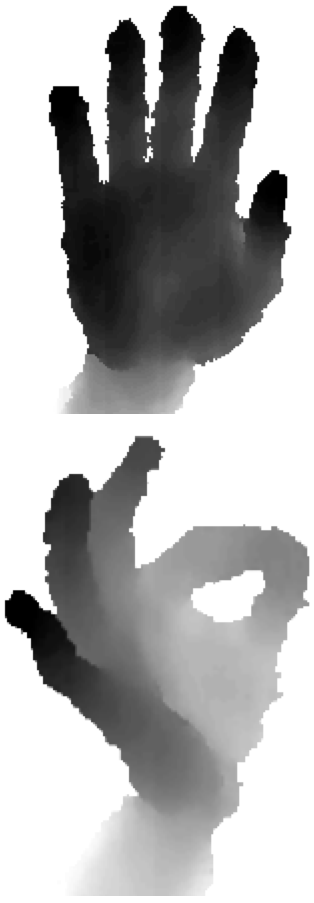
\includegraphics[width=0.75\textwidth]{figures_1_hand_tracking/Kinect_tiled}
                \caption{\footnotesize Sensor Depth}
        \end{subfigure}
        \begin{subfigure}{0.25\textwidth}
                \centering
                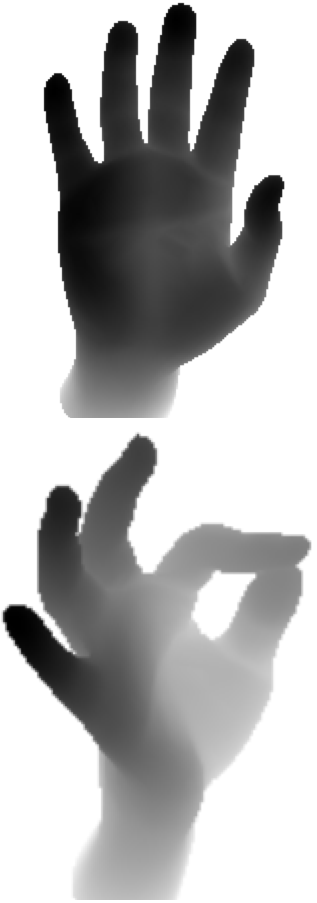
\includegraphics[width=0.75\textwidth]{figures_1_hand_tracking/Synthetic_tiled}
                \caption{\footnotesize Synthetic Depth}
        \end{subfigure}
        \begin{subfigure}{0.25\textwidth}
                \centering
                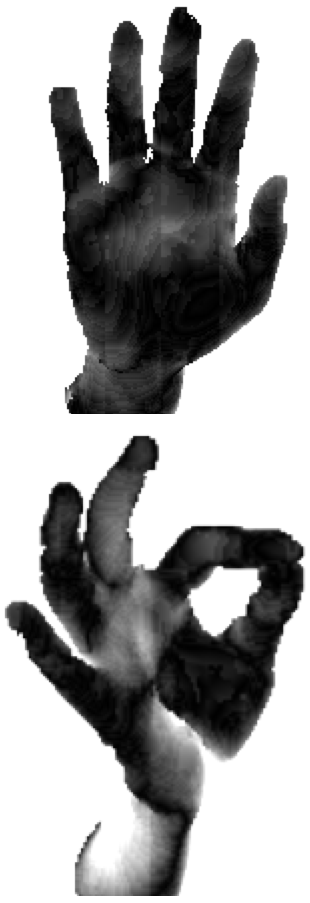
\includegraphics[width=0.75\textwidth]{figures_1_hand_tracking/Residue_tiled}
                \caption{\footnotesize Per-Pixel Error}
        \end{subfigure}
        \caption{Dataset Creation: Objective Function Data (with Libhand model~\protect\cite{libhand})}
        \label{fig:pso}
\end{figure}

Since we do not have a ground-truth measure for the 42 DOF hand model fitting, quantitative evaluation of this stage is difficult. \emph{Qualitatively}, the fitting accuracy was visually consistent with the underlying point cloud. An example of a fitted frame is shown in Figure \ref{fig:pso}. Only a very small number of poses failed to fit correctly; for these difficult poses, manual intervention was required.

One limitation of this system was that the frame rate of the PrimeSense camera (30fps) was not enough to ensure sufficient temporal coherence for correct convergence of the PSO optimizer. To overcome this, we had each user move their hands slowly during training data capture. Using a workstation with an Nvidia GTX 580 GPU and 4 core Intel processor, fitting each frame required 3 to 6 seconds. The final database consisted of 76,712 training set images, 2,421 validation set images and 2,000 test set images with their corresponding heat-maps, collected from multiple participants. A small sample of the test set images is shown in Figure \ref{fig:cnn_training_set_images}.

\begin{figure}[ht]
\centering
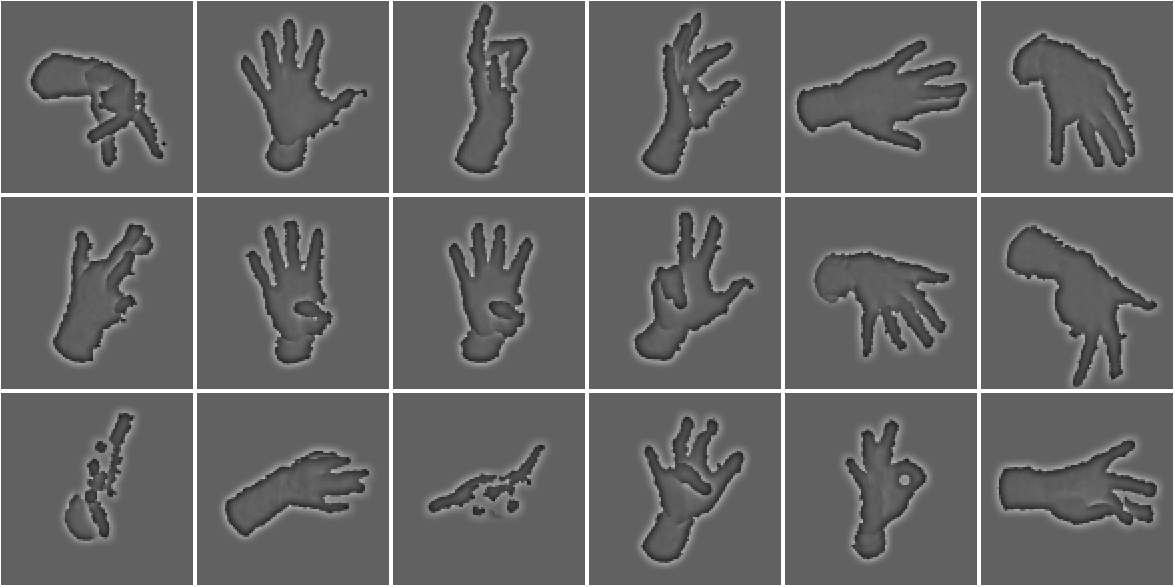
\includegraphics[width=0.8\columnwidth]{figures_1_hand_tracking/train_data_3_6}
    \caption{Sample ConvNet Test Set images}
    \label{fig:cnn_training_set_images}
\end{figure}

The ConvNet training took approximately 24 hours where early stopping is performed after 350 epochs to prevent overfitting. ConvNet hyper parameters, such as learning rate, momentum, L2 regularization, and architectural parameters (e.g., max-pooling window size or number of stages) were chosen by coarse meta-optimization to minimize a validation-set error. 2 stages of convolution (at each resolution level) and 2 fully-connected neural network stages were chosen as a tradeoff between numerous performance characteristics: generalization performance, evaluation time, and model complexity (or ability to infer complex poses). Figure \ref{fig:conv_learning_graph} shows the mean squared error (MSE) after each epoch. The MSE was calculated by taking the mean of sum-of-squared differences between the calculated 14 feature maps and the corresponding target feature maps.

\begin{figure}[ht]
\centering
\includegraphics[width=0.5\textwidth]{figures_1_hand_tracking/conv_learning_graph.pdf}
    \caption{ConvNet Learning Curve}
    \label{fig:conv_learning_graph}
\end{figure}

The mean UV error of the ConvNet heat-map output on the test set data was 0.41px (with standard deviation of 0.35px) on the 18x18 resolution heat-map image\footnote{To calculate this error we used the technique described in Section \ref{sec:realtimeposedetection} to calculate the heat-map UV feature location and then calculated the error distance between the target and ConvNet output locations}. After each heat-map feature was translated to the 640x480 depth image, the mean UV error was 5.8px (with standard deviation of 4.9px). Since the heat-map downsampling ratio is depth dependent, the UV error improves as the hand approaches the sensor. For applications that require greater accuracy, the heat-map resolution can be increased for better spatial accuracy at the cost of increased latency and reduced throughput.

\begin{table}[h]
\small
\centering
\begin{tabular}{lcc}
        \hline
        Feature Type           & Mean (px) & STD (px) \\
        \hline
        Palm                   & 0.33       & 0.30      \\
        Thumb Base \& Knuckle  & 0.33       & 0.43      \\
        Thumb Tip              & 0.39       & 0.55      \\
        Finger Knuckle         & 0.38       & 0.27      \\
        Finger Tip             & 0.54       & 0.33      \\
        \hline
    \end{tabular}
\caption{Heat-Map UV Error by Feature Type}
\label{tab:uv_errors}
\end{table}

Table~\ref{tab:uv_errors} shows the UV accuracy for each feature type. Unsurprisingly, we found that the ConvNet architecture had the most difficulty learning fingertip positions, where the mean error is 61\% higher than the accuracy of the palm features. The likely cause for this inaccuracy is twofold. Firstly, the fingertip positions undergo a large range of motion between various hand-poses and therefore the ConvNet must learn a more difficult mapping between local features and fingertip positions. Secondly, the PrimeSense Carmine 1.09 depth camera cannot always recover depth of small surfaces such as fingertips. The ConvNet is able to learn this noise behavior, and is actually able to approximate fingertip location in the presence of missing data, however the accuracy for these poses is low.

The computation time of the entire pipeline is 24.9ms, which is within our 30fps performance target. Within this period: decision forest evaluation takes 3.4ms, depth image preprocessing takes 4.7ms, ConvNet evaluation takes 5.6ms and pose estimation takes 11.2ms. The entire pipeline introduces approximately one frame of latency. For an example of the entire pipeline running in real-time as well as puppeteering of the LBS hand model, please refer to the supplementary video (screenshots from this video are shown in Figure~\ref{fig:screenshots}).

\begin{figure}[ht]
\centering
        \begin{subfigure}{0.3375\textwidth}
                \centering
                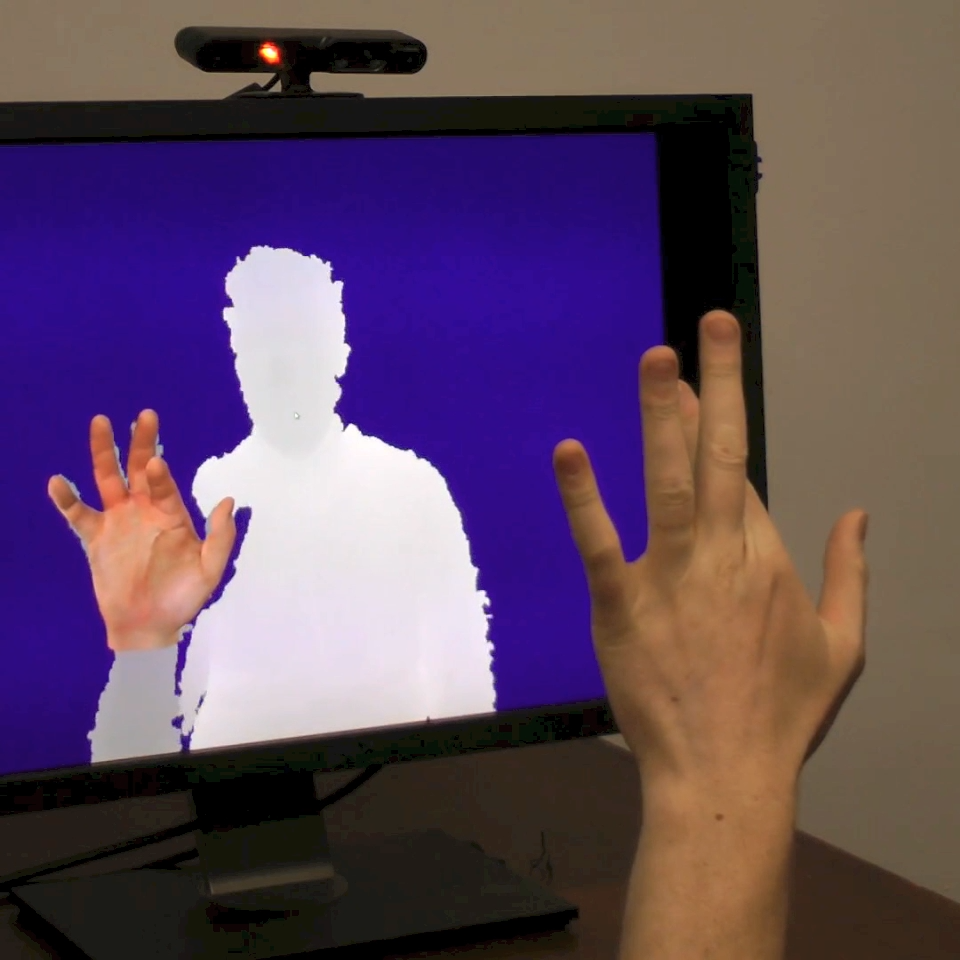
\includegraphics[width=\textwidth]{figures_1_hand_tracking/screenshot1_clipped}
                \caption{\footnotesize }
        \end{subfigure}
        \begin{subfigure}{0.28125\textwidth}
                \centering
                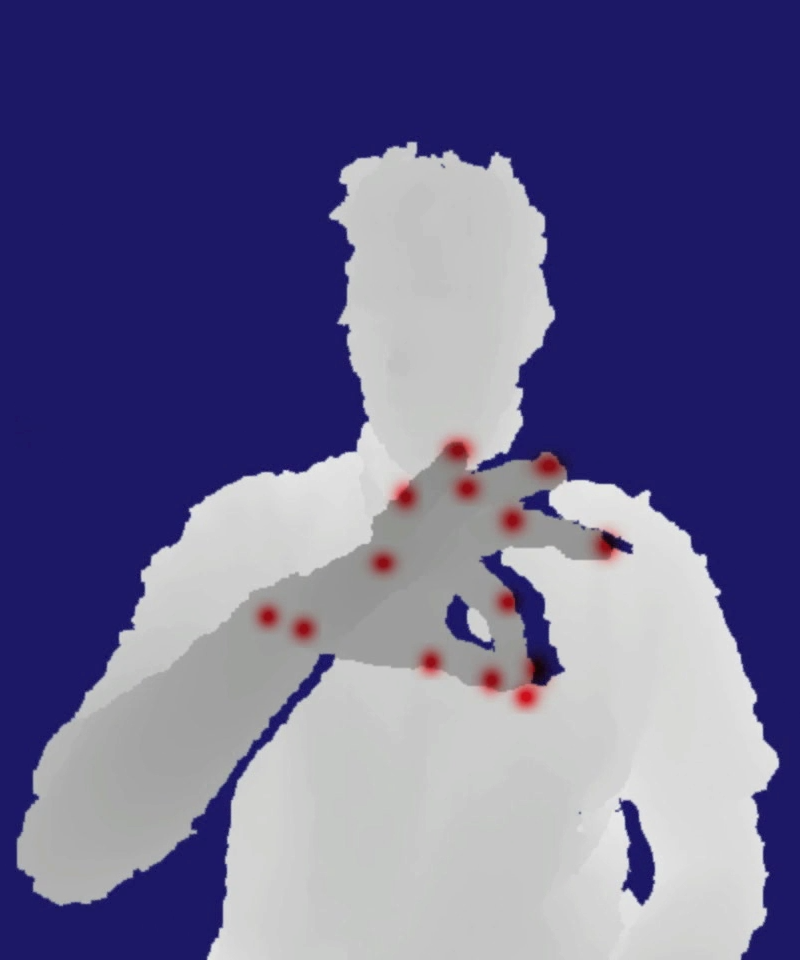
\includegraphics[width=\textwidth]{figures_1_hand_tracking/screenshot2_clipped}
                \caption{\footnotesize }
        \end{subfigure}
        \begin{subfigure}{0.28125\textwidth}
                \centering
                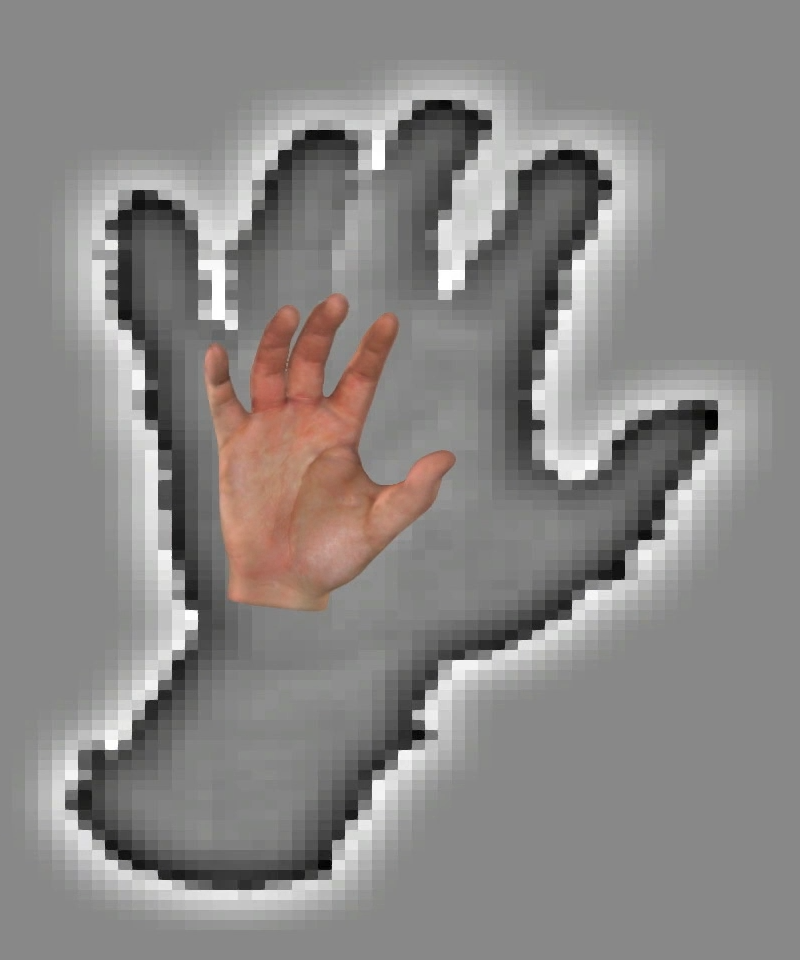
\includegraphics[width=\textwidth]{figures_1_hand_tracking/screenshot3_clipped}
                \caption{\footnotesize }
        \end{subfigure}
        \caption{Real-Time Tracking Results, a) Typical Hardware Setup, b) Depth with Heat-Map Features, c) ConvNet Input and Pose Output}
        \label{fig:screenshots}
\end{figure}

Figure~\ref{fig:fail_cases} shows three typical fail cases of our system. In \ref{fig:fail_cases}a) finite spatial precision of the ConvNet heat-map results in finger tip positions that are not quite touching. In \ref{fig:fail_cases}b) no similar pose exists in the database used to train the ConvNet, and for this example the network generalization performance was poor. In \ref{fig:fail_cases}c) the PrimeSense depth camera fails to detect the ring finger (the surface area of the finger tip presented to the camera is too small and the angle of incidence in the camera plane is too shallow), and the ConvNet has difficulty inferring the finger tip position without adequate support in the depth image, which results in an incorrect inferred position.

\begin{figure}[ht]
\centering
    \renewcommand{\tabcolsep}{0.02\linewidth}
    \begin{tabular}{ccc}
        \adjustbox{valign=m}{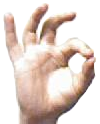
\includegraphics[width=0.2\linewidth]{figures_1_hand_tracking/fail_case0_rgb_clipped.png}} & \adjustbox{valign=m}{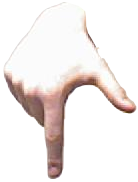
\includegraphics[width=0.2\linewidth]{figures_1_hand_tracking/fail_case1_rgb_clipped.png}} & \adjustbox{valign=m}{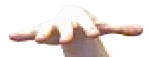
\includegraphics[width=0.2\linewidth]{figures_1_hand_tracking/fail_case2_rgb_clipped.png}} \\
        \adjustbox{valign=m}{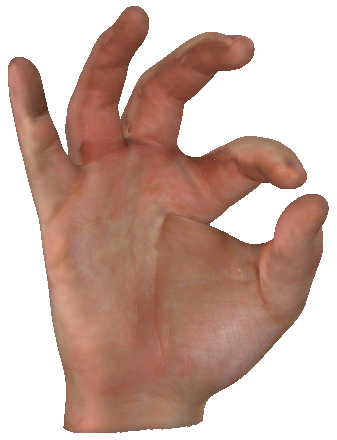
\includegraphics[width=0.2\linewidth]{figures_1_hand_tracking/fail_case0_model_clipped.png}} & \adjustbox{valign=m}{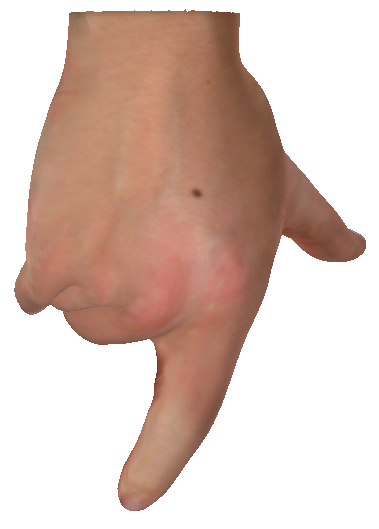
\includegraphics[width=0.2\linewidth]{figures_1_hand_tracking/fail_case1_model_clipped.png}} & \adjustbox{valign=m}{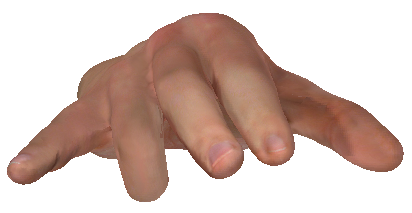
\includegraphics[width=0.2\linewidth]{figures_1_hand_tracking/fail_case2_model_clipped.png}} \\
        a) & b) & c)
    \end{tabular}
    \caption{Fail Cases: RGB ground-truth (top row), inferred model~\protect\cite{libhand} pose (bottom row)}
    \label{fig:fail_cases}
\end{figure}

Figure~\ref{fig:users} shows that the ConvNet output is tolerant for hand shapes and sizes that are not well represented in the ConvNet training set. The ConvNet and RDF training sets did not include any images for user b) and user c) (only user a)). We have only evaluated the system's performance on adult subjects. We found that adding a single per-user scale parameter to approximately adjust the size of the LBS model to a user's hand, helped the real-time IK stage better fit to the ConvNet output.

\begin{figure}[ht]
\centering
    \renewcommand{\tabcolsep}{0.006\linewidth}
    \begin{tabular}{ccc}
        % The SUM of all three image widths needs to be 0.31 * 3 \linewidth
        % User 1: 1136x1000 (rgb & depth) = 31.94% --> Width = 0.2970\linewidth
        % User 2: 1239x1000 (rgb & depth) = 34.83% --> Width = 0.3239\linewidth
        % User 3: 1182x1000 (rgb & depth) = 33.23% --> Width = 0.3090\linewidth
        % Total = 3557
        \adjustbox{valign=m}{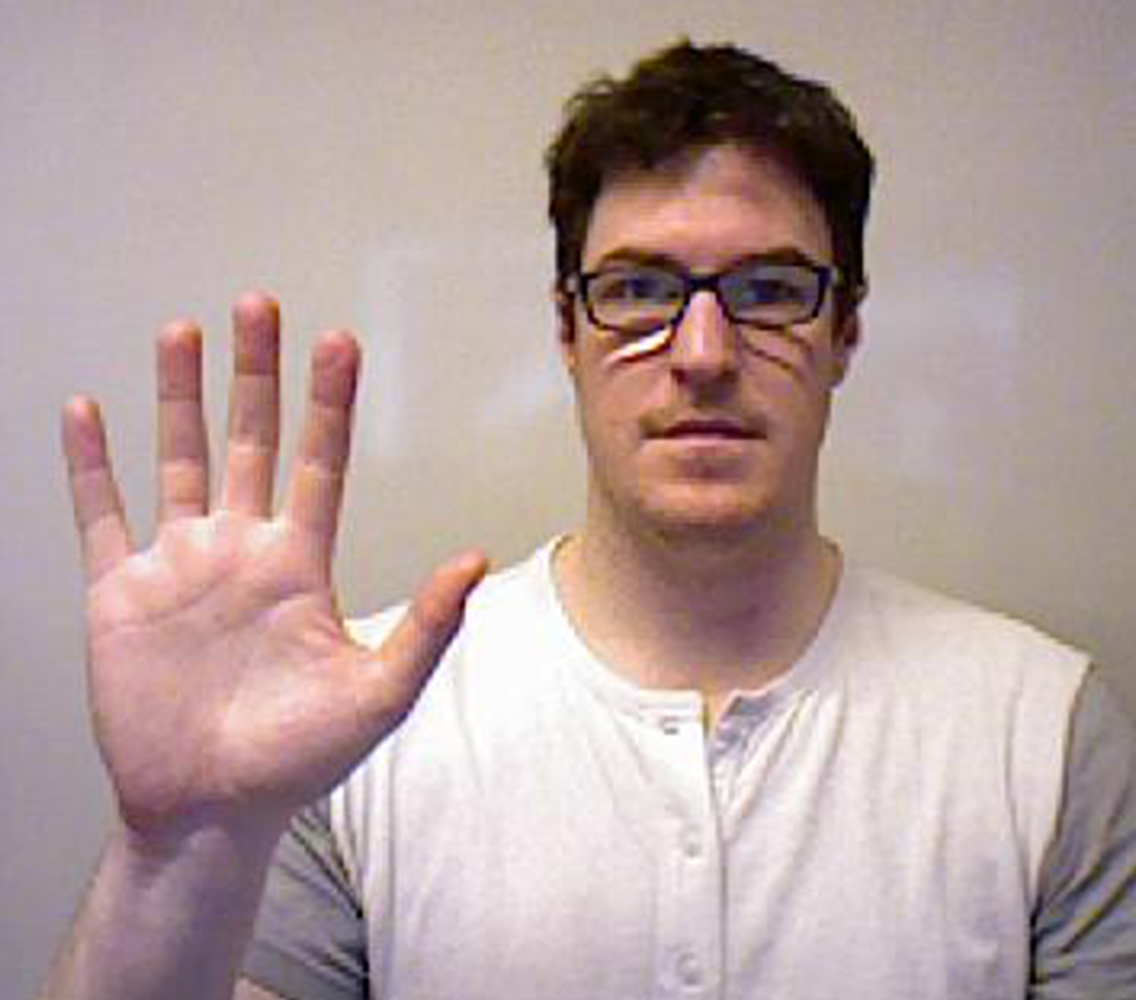
\includegraphics[width=0.2970\linewidth]{figures_1_hand_tracking/user1_rgb_cropped.png}} & \adjustbox{valign=m}{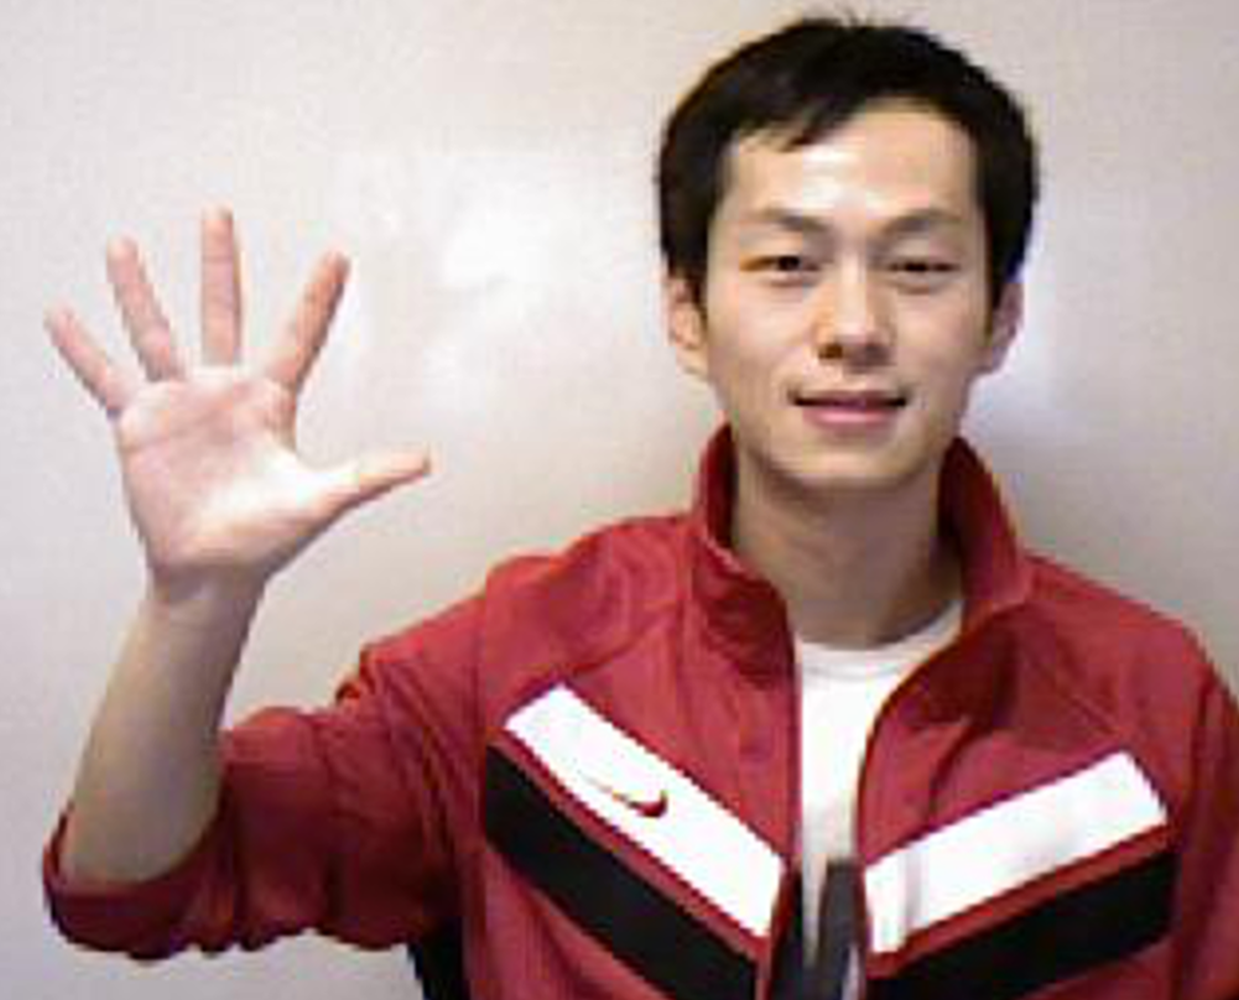
\includegraphics[width=0.3239\linewidth]{figures_1_hand_tracking/user2_rgb_cropped.png}} & \adjustbox{valign=m}{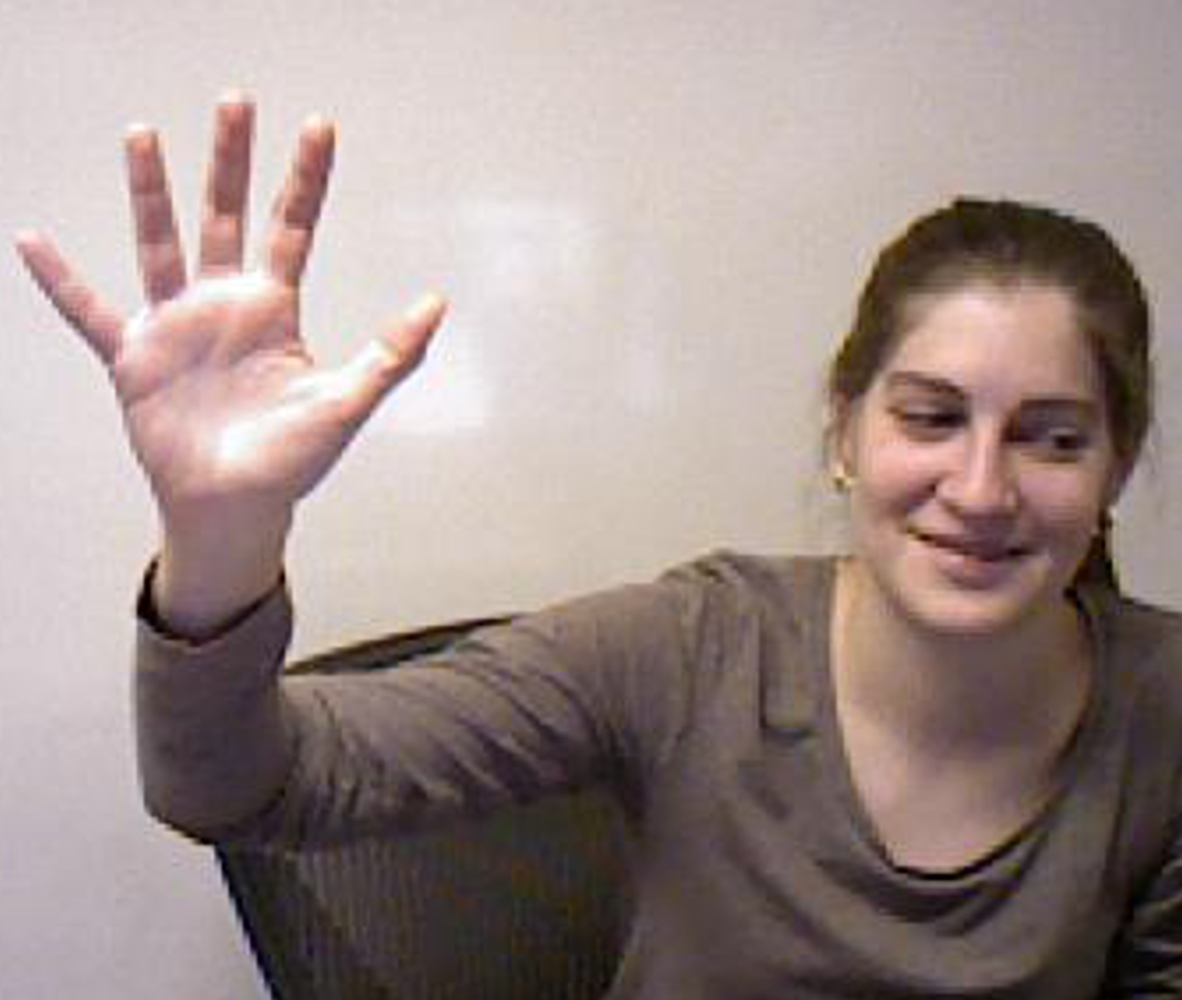
\includegraphics[width=0.3090\linewidth]{figures_1_hand_tracking/user3_rgb_cropped.png}} \\[0.98cm]
        \adjustbox{valign=m}{\includegraphics[width=0.2970\linewidth]{figures_1_hand_tracking/user1_depth_cropped_annotated.pdf}} & \adjustbox{valign=m}{\includegraphics[width=0.3239\linewidth]{figures_1_hand_tracking/user2_depth_cropped_annotated.pdf}} & \adjustbox{valign=m}{\includegraphics[width=0.3090\linewidth]{figures_1_hand_tracking/user3_depth_cropped_annotated.pdf}} \\[0.98cm]
        a) & b) & c)
    \end{tabular}
    \caption{Hand Shape/Size Tolerance: RGB ground-truth (top row), depth with annotated ConvNet output positions (bottom row)}
    \label{fig:users}
\end{figure}

Comparison of the relative real-time performance of this work with relevant prior art, such as that of \cite{3Gear} and \cite{Melax:2013}, is difficult for a number of reasons. Firstly, \cite{Melax:2013} uses a different capture device, which prevents fair comparison as it is impossible (without degrading sensor performance by using mirrors) for multiple devices to see the hand from the same viewpoint simultaneously. Secondly, no third-party ground truth database of poses with depth frames exists for human hands, so comparing the quantitative accuracy of numerous methods against a known baseline is not possible. More importantly however, is that the technique utilized by \cite{3Gear} is optimized for an entirely different use case and so fair comparison with their work is very difficult. \cite{3Gear} utilizes a vertically mounted camera, can track multiple hands simultaneously, and is computationally less expensive than the method presented in our work.

Figure~\ref{fig:compare} examines the performance of this work with the proprietary system of \cite{3Gear} (using the fixed-database version of the library), for 4 poses chosen to highlight the relative difference between the two techniques (images used with permission from 3Gear). We captured this data by streaming the output of both systems simultaneously (using the same RGBD camera). We mounted the camera vertically, as this is required for \cite{3Gear}, however our training set did not include any poses from this orientation.
Therefore, we expect our system to perform sub-optimally for this very different use case.

\begin{figure}[ht]
\centering
    \renewcommand{\tabcolsep}{0.006\linewidth}
    \resizebox{\linewidth}{!}{%
    \begin{tabular}{cccc}
        % The SUM of all four image widths needs to be (1 - 0.006 * 4) = 0.976 \linewidth
        % Pose A: 460x512 (rgb & depth) = 23.69% --> Width = 0.2312\linewidth
        % Pose B: 489x512 (rgb & depth) = 25.18% --> Width = 0.2457\linewidth
        % Pose C: 579x512 (rgb & depth) = 29.81% --> Width = 0.2910\linewidth
        % Pose D: 414x512 (rgb & depth) = 20.81% --> Width = 0.2081\linewidth
        % Total = 1942
        \adjustbox{valign=m}{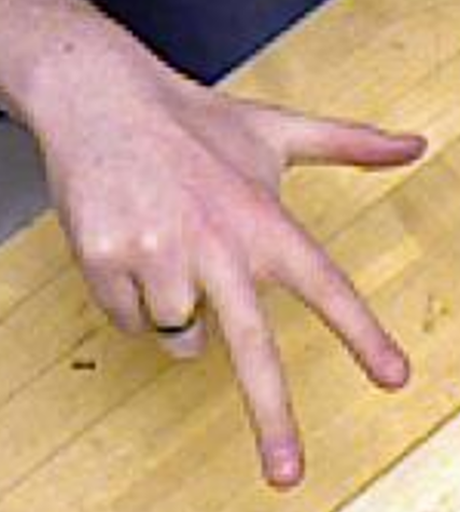
\includegraphics[width=0.2312\linewidth]{figures_1_hand_tracking/compare_a_rgb_cropped.png}} & \adjustbox{valign=m}{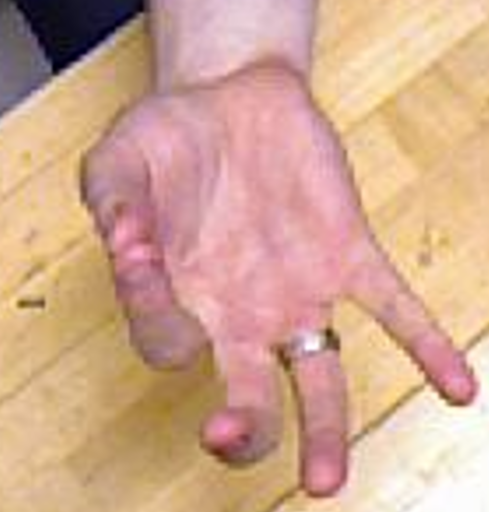
\includegraphics[width=0.2457\linewidth]{figures_1_hand_tracking/compare_b_rgb_cropped.png}} & \adjustbox{valign=m}{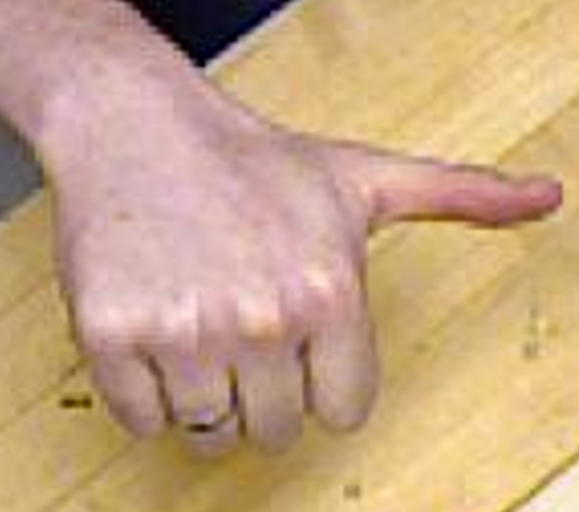
\includegraphics[width=0.2910\linewidth]{figures_1_hand_tracking/compare_c_rgb_cropped.png}} & \adjustbox{valign=m}{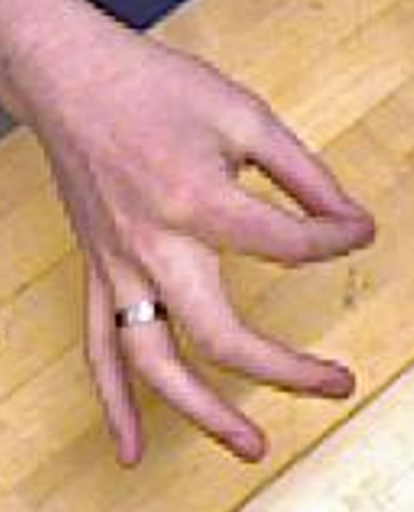
\includegraphics[width=0.2081\linewidth]{figures_1_hand_tracking/compare_d_rgb_cropped.png}} \\[0.98cm]
        \adjustbox{valign=m}{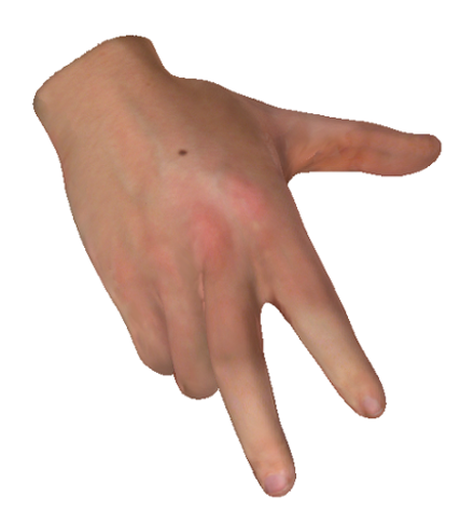
\includegraphics[width=0.2312\linewidth]{figures_1_hand_tracking/compare_a_ours_cropped.png}} & \adjustbox{valign=m}{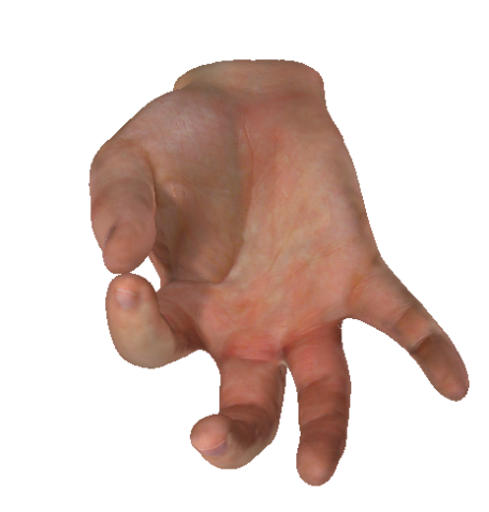
\includegraphics[width=0.2457\linewidth]{figures_1_hand_tracking/compare_b_ours_cropped.png}} & \adjustbox{valign=m}{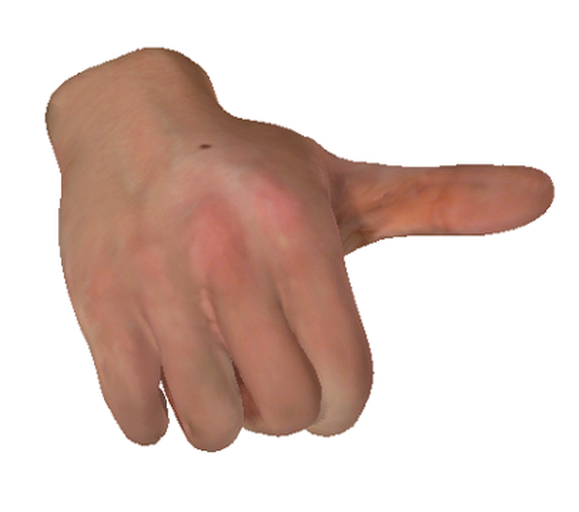
\includegraphics[width=0.2910\linewidth]{figures_1_hand_tracking/compare_c_ours_cropped.png}} & \adjustbox{valign=m}{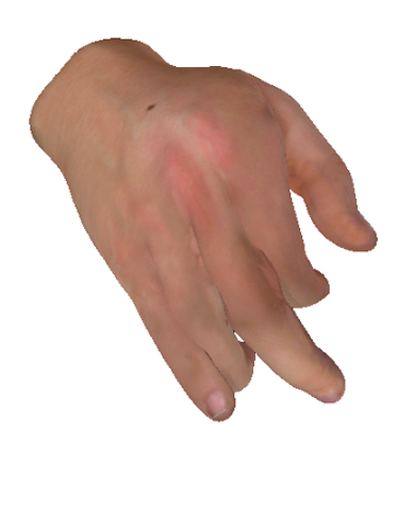
\includegraphics[width=0.2081\linewidth]{figures_1_hand_tracking/compare_d_ours_cropped.png}} \\[0.98cm]
        \adjustbox{valign=m}{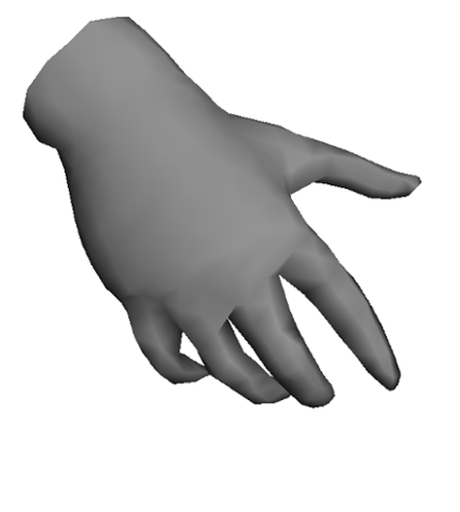
\includegraphics[width=0.2312\linewidth]{figures_1_hand_tracking/compare_a_theirs_cropped.png}} & \adjustbox{valign=m}{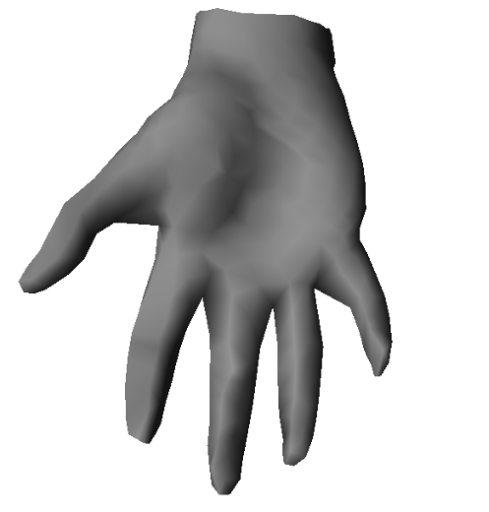
\includegraphics[width=0.2457\linewidth]{figures_1_hand_tracking/compare_b_theirs_cropped.png}} & \adjustbox{valign=m}{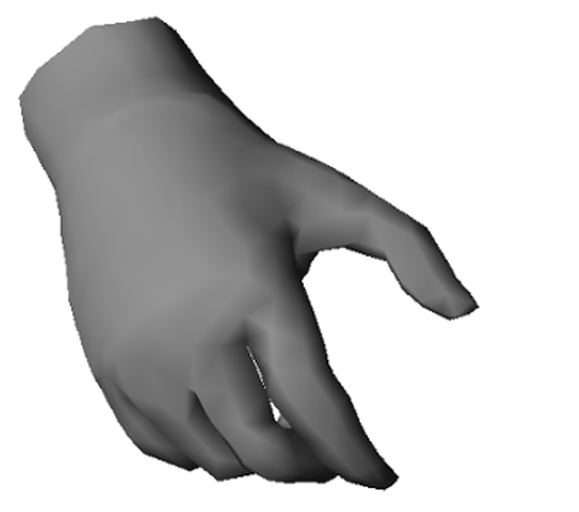
\includegraphics[width=0.2910\linewidth]{figures_1_hand_tracking/compare_c_theirs_cropped.png}} & \adjustbox{valign=m}{\includegraphics[width=0.2081\linewidth]{figures_1_hand_tracking/compare_d_theirs_cropped.png}} \\[0.98cm]
        a) & b) & c) & d)
    \end{tabular}
    } % end resizebox
    \caption{Comparison with state-of-the-art commercial system: RGB ground-truth (top row), this work inferred model~\protect\cite{libhand} pose (middle row), \protect\cite{3Gear} inferred model pose (bottom row) (images used with permission from 3Gear).}
    \label{fig:compare}
\end{figure}

\section{Future Work}
\label{sec:future_work}

As indicated in Figure~\ref{fig:users}, qualitatively we have found that the ConvNet generalization performance to varying hand shapes is acceptable but could be improved. We are confident we can make improvements by adding more training data from users with different hand sizes to the training set.

For this work, only the ConvNet forward propagation stage was implemented on the GPU. We are currently working on implementing the entire pipeline on the GPU, which should improve performance of the other pipeline stages significantly. For example, the GPU ConvNet implementation requires 5.6ms, while the same network executed on the CPU (using optimized multi-threaded C++ code) requires 139ms.

The current implementation of our system can track two hands only if they are not interacting. While we have determined that the dataset generation system can fit multiple strongly interacting hand poses with sufficient accuracy, it is future work to evaluate the neural network recognition performance on these poses. Likewise, we hope to evaluate the recognition performance on hand poses involving interactions with non-hand objects (such as pens and other man-made devices).

While the pose recovery implementation presented in this work is fast, we hope to augment this stage by including a model-based fitting step that trades convergence radius for fit quality. Specifically, we suspect that replacing our final IK stage with an energy-based local optimization method, inspired by the work of Li et al.~\cite{li08global} could allow our method to recover second-order surface effects such as skin folding and skin-muscle coupling from very limited data, and still with low-latency. In addition to inference, such a localized energy-minimizing stage would enable improvements to the underlying model itself. Since these localized methods typically require good registration, our method, which gives correspondence from a single image could advance the state-of-the-art in non-rigid model capture.

Finally, we hope to augment our final IK stage with some form of temporal pose prior to reduce jitter; for instance, using an extended Kalman filter as a post-processing step to clean up the ConvNet feature output.
